Inspired by the FloPoCo~\cite{8877424} project, our design methodology can best be described as \emph{computing just right}.
We aim for just the right amount of compute and abstraction for the task at hand, no more no less.
This methodology stands in contrast to the design methodologies of architecture designers for commodity hardware accelerators (such as GPUs), which aim to support a large set of use cases.
Accordingly, our methodology consists of five techniques distilled from such general purpose architectures and tools but simplified for our specific purposes.

\subsection{Abstract Interpretation for Efficient Transformations}\label{subsec:loop-unrolling}

It is well known that the most straightforward way to achieve lowest latency inference of a DNN is to linearize the control flow graph~\cite{osti_1574050} (i.e., remove branches) and flatten the dataflow graph as much as possible~\cite{10.1145/3295500.3356173} (i.e., execute as many operations in parallel as possible).
For intermediate level representations of a DNN this corresponds to loop unrolling followed by fusion (alternatively known as unroll and jam~\cite{thomas1971catalogue}).
For example, consider the pair of loop nests in Listing~\ref{lst:loop_fusion}.
Note that a loop fusion pass performed by either MLIR or LLVM would verify that memory independence constraints are satisfied for all pairs of stores and loads in each of the loop nests.
Thus, after unrolling the inner loops of the second loop nest (on \mintinline{mlir}{%arg5}, \mintinline{mlir}{%arg6}, \mintinline{mlir}{%arg7}) we incur
\[
	\mathtt{\%c1} \times \mathtt{\%c3} \times \mathtt{\%c3} \times 2 \times 4
\]
memory independence checks.
Thus, unroll and fuse optimizations take increasingly longer as one experiments with larger and larger unroll thresholds; the \emph{unroll threshold} determines which loops will be fully unrolled (all loops with trip count less than or equal to the threshold will be unrolled).
\begin{longlisting}
	\inputminted[highlightlines={5,6,17,18,19,22}]{mlir}{sources/loop_fusion.mlir}
	\caption{Loop fusion and unrolling example, with \hl{emphasis} on loads and stores whose independence must verified.}
	\label{lst:loop_fusion}
\end{longlisting}
\begin{longlisting}
	\inputminted[highlightlines={5,6,11-13,16},linenos=true,numbersep=\mintednumbersep]{mlir}{sources/unrolled_loop.mlir}
	\caption{Unrolled and fused loop, for which store-load forwarding can be performed.}
	\label{lst:storeloadforwarding}
\end{longlisting}

%followed by store-load forwarding or, alternatively, wholly promoting stores-loads to registers.
Following unroll and jam, we are able to perform \emph{store-load forwarding}, i.e., we are able to omit those store operations that store to memory addresses which are subsequently loaded from (with no intervening stores).
For example, consider the above loop nests fused, with the second loop nest having the inner three loops fully unrolled (see Listing~\ref{lst:storeloadforwarding}); the store operations on lines 6 and 13 can be entirely eliminated and the load operation on line 5 can be forwarded to the \inlinemlir{arith.addf} on line 15.
For each load operation that follows a store operation, a compiler must check whether the store and the load access the same location in memory, and further verify that there are no intervening store operations to the same memory address;
with respect to correctness, this requires solving a system of constraints~\cite{10.2307/2322281}.
We observe that as loops are further and further unrolled, the cost of this particular optimization grows polynomially; consider a fully unrolled loop nest, with many parallel dataflows, for which a store operation in one dataflow might be forwarded across a parallel dataflow (and thus incur checks against all stores and loads in that parallel dataflow).

In principle, we might rely on MLIR or LLVM to perform each of these optimization passes.
The chief impediment to relying on these general purpose compilers for our needs is the runtime complexity of the their implementations.
Note that for general purpose programs this is an acceptable cost, especially given that most development is done without these optimization (leaving the aggressive optimizations for release ready builds).
For us, given that the logic and dataflow of BraggNN is fixed (having already been iterated on), and given that we are in fact searching the design space for optimal low-level representations of the DNN, the runtimes of these optimization passes are prohibitive (taking on the order of hours and sometimes days to complete).
Moreover, often their rigor and conservatism are unnecessary given a high-level understanding of the structure of BraggNN; for example, in the case of fully unrolling the above loop nests (forwarding from the stores during initialization to the loads during accumulation), the region within which the forward is safe is clear from the semantics of convolutions.
The loop indices and corresponding memory addresses for these safe store-load forwards are very easy to compute analytically and ahead of time (even in the presence of complications such as strided tensors).

In order to avoid the runtime costs associated with these unnecessarily conservative optimization passes, we omit them.
Instead, we do not lower BraggNN past the structured control flow (\inlinemlir{scf}) dialect in MLIR, and instead implement an abstract interpreter, which effectively performs the unrolling by ``running'' BraggNN with alternative semantics (see Eqns~\eqref{eqn:semantics}).
In addition to efficiently unrolling loop nests, our abstract interpreter performs store-load forwarding.
We also reinterpret remaining stores and loads to memory as reads and writes to registers, thus simplifying our design; such stores and loads would otherwise translate to stores and loads from Block RAM (BRAM).
Furthermore, since BraggNN is a relatively small DNN, we inline absolutely all of the weight tensors as constants and perform \emph{constant propagation}.
Finally, our abstract interpreter identifies sequences of multiplications and additions and groups them together such that they can be scheduled to reuse accumulator registers (effectively forming a multiply-accumulator); this grouping is the chief optimization that enables us to efficiently map BraggNN to FPGA.
In summary we perform the following transformations on the \inlinemlir{scf} representation of BraggNN:
\begin{enumerate}
	\item We completely eliminate any latency due to loading from or storing to BRAM for intermediate activations;
	\item We completely eliminate all logic (i.e., integer arithmetic) related to calculating memory offsets, a non-trivial reduction in instruction count and design complexity (see figure <figure> for reduction in instruction count);
	\item We instantiate a reduced set of floating point operation cores, and thus reduce complexity and overall latency of our design.
\end{enumerate}
Note, we are able to perform the memory to registers promotions owing to the fact that BraggNN is a relatively compact DNN and our target FPGA is plentiful in registers.
The reinterpreted semantics implemented by our abstract interpreter are presented in Eqns~\eqref{eqn:semantics}.

\begin{figure}
	\begin{equation}\label{eqn:semantics}
		\begin{split}
			f_{Z} \llbracket x \coloneqq y + z\rrbracket (\sigma) &= [ x \mapsto Z ] (\sigma) \\
			f_{Z} \llbracket x \coloneqq y + z\rrbracket (\sigma) &= [ x \mapsto Z ] (\sigma) \\
			f_{Z} \llbracket x \coloneqq y + z\rrbracket (\sigma) &= [ x \mapsto Z ] (\sigma) \\
		\end{split}
	\end{equation}
	\caption{This is a placeholder.}\label{fig:semantics}
\end{figure}

\subsection{Parallel Topological Sort Scheduling}\label{subsec:parallel-toposort-scheduling}

In addition to reducing the runtime of the compiler frontend, our abstract interpreter simplifies the representation such that we may emit a simplified LLVM IR pass to Vitis HLS, and thus, in theory reduce its runtime as well.
In actuality, performing these optimizations has no effect on the runtime of Vitis HLS, since it will rerun the same (or similar) passes as part of its transformation pipeline.
Thus, a fundamental challenge in implementing BraggNN as a digital design is reducing the time taken by Vitis HLS in performing its own optimizations; in addition to those ultimately redundant optimizations, Vitis' HLS scheduling algorithms takes an inordinate amount of time to schedule the large number of operations that comprise BraggNN when fully unrolled, even after eliding unnecessary operations (such as the integer arithmetic associated with computing memory offsets).

Thus it becomes necessary to completely eliminate Vitis and (therefore HLS) from the design process.
Recall that the critical function which Vitis HLS fulfills is the scheduling of operations during each clock cycle, in such a way that they respect the dataflow graph of BraggNN; that schedule then informs the construction of a corresponding FSM.
In general, for complex programs, this is indeed a computationally intensive task, necessitating formulating the scheduling problem and solving it using either an integer programming solver or, if the problem is formulated as an SDC, an LP solver.
In the case of BraggNN, and in fact many DNNs, where the dataflow is very regular and where parallel execution is only bounded by the number of DSPs (assuming BRAM access is eliminated), it is straightforward to construct the optimal schedule based solely on a topological sort of the operations.

In fact, by computing the schedule ``by hand'', we can exercise more precise control over DSP usage and thus further reduce the overall complexity of the design.
That it to say, we can schedule using the maximum number of DSPs possible during each state of the FSM, in contrast to Vitis HLS, which attempts to make conservative use of DSPs (which leads to excessive LUT usage to support time multiplexing of the DSPs); see figure <...> for a comparison the LUT usage using our scheduling algorithm versus Vitis HLS scheduling algorithm.
One thing to note here is that computing a schedule even just using sequential topological sort becomes costly (in terms of runtime) for the larger scalings of BraggNN, where we need to schedule upwards of 1E6 operations.
To mitigate these costs as well (in order to enable fast iteration on design choices) we implement a parallelized topological sort~\cite{sanders2019sequential}.
See Algorithm~\ref{alg:toposort} for a specification of our scheduling algorithm.

\begin{algorithm}
	\caption{Placeholder}\label{alg:toposort}
	\begin{algorithmic}
		\Require $n \geq 0$
		% \Ensure $y = x^n$
		% \State $y \gets 1$
		% \State $X \gets x$
		% \State $N \gets n$
		% \While{$N \neq 0$}
		% \If{$N$ is even}
		% \State $X \gets X \times X$
		% \State $N \gets \frac{N}{2}$  \Comment{This is a comment}
		% \ElsIf{$N$ is odd}
		% \State $y \gets y \times X$
		% \State $N \gets N - 1$
		% \EndIf
		% \EndWhile
	\end{algorithmic}
\end{algorithm}

\subsection{Bit Twiddling Hacks}\label{subsec:bit-twiddling-hacks}

FPGAs do not permit dynamic reconfiguration of DSPs to support fully heterogeneous operations; a set of DSPs associated with floating point addition can be dynamically reconfigured to perform subtraction but multiplication (likewise vice-versa).
Thus, in order to maximize reuse of DSPs we only instantiate floating point IP cores for multiplication.
We map the remaining operations necessitated by BraggNN (\inlinemlir{fsub}, \inlinemlir{fexp}, \inlinemlir{relu}, \inlinemlir{fdiv}) to (\inlinemlir{fmul}) and addition (\inlinemlir{fadd}).
For the cases of \inlinemlir{fsub} and \inlinemlir{fexp} this is straightforward (a bit flip on the sign bit to handle the former and a Taylor series expansion to handle \inlinemlir{fexp}).
For the case of \inlinemlir{relu}, note that for a IEEE 754 $n$-bit floating point number $x$
$$
\max(0, x) = x \iff x[0] = 0
$$
where $x[0]$ represents the sign bit of $x$.
Division is the only primitive operation that presents a serious challenge to normalization in this way.
To represent division (in terms of \inlinemlir{fmul}) we exploit the fact that aliasing a floating point number as an integer effectively calculates the approximate binary logarithm~\cite{enwiki:1081681080} of the number;
we use this property to approximate the inverse (of a floating point number) and then perform division through multiplication by that inverse.
In our experiments (and prior work~\cite{10.1007/978-0-387-72258-0_14}) this approximation incurs approximately a $4\%$ difference in accuracy per division.

Finally, we experiment with alternative bitwidth implementations of IEEE754 floating point.
With respect to the BraggNN training, we observe that the sample data does not use a full 8 bit exponent (see Figure~\ref{fig:numexp}).
\begin{figure}
	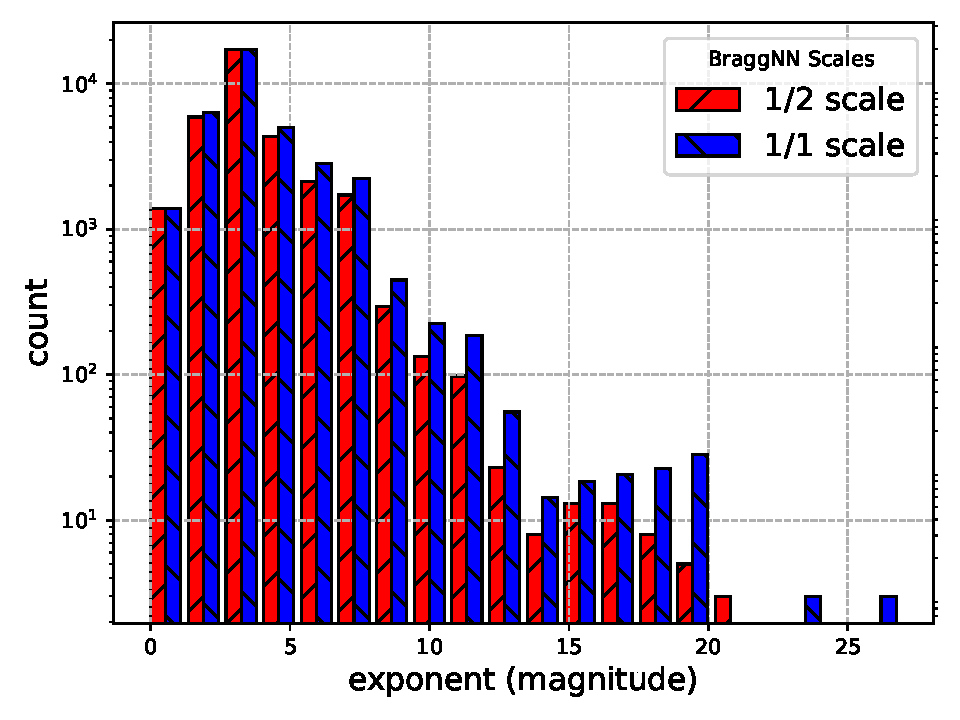
\includegraphics[width=\columnwidth]{figures/exp_hist}
	\caption{Range of exponent values for BraggNN weights.}\label{fig:numexp}
\end{figure}
With this in mind, we deploy BraggNN using half precision floats, i.e., using 5 bits to represent the exponent and 11 bits to represent the mantissa.
This produces floating point arithmetic cores that use fewer registers, LUTs, and having smaller wire delays, again leading to a reduction in overall complexity and end to end latency.
